\documentclass[12pt, a4paper, oneside]{scrartcl}

\usepackage[utf8]{inputenc}
\usepackage[T1]{fontenc}
\usepackage[ngerman]{babel}

\usepackage[T1]{fontenc}
\usepackage{caladea} % close enough für Cambria :clueless:

\usepackage{geometry}

\usepackage[ngerman]{babel}
\usepackage{csquotes}
\usepackage[
    backend=biber,
    style=verbose,
    giveninits=true,
    uniquename=init,
    citestyle=authoryear,
]{biblatex}

\addbibresource{Quellen.bib}
    
\geometry{
    a4paper,
    top=2.5cm,
    bottom=2.5cm,
    left=2.5cm,
    right=2.5cm
}

\usepackage{setspace}
\onehalfspacing

\usepackage{ragged2e}

\usepackage{indentfirst}

\usepackage{graphicx}
\usepackage{amsmath}
\usepackage{amsfonts}
\usepackage{amssymb}

\usepackage{float}

\usepackage{xcolor}
\usepackage{hyperref}
\hypersetup{
    colorlinks=true,
    linkcolor=black,
    citecolor=black,
    filecolor=black,
    urlcolor=blue,
    pdftitle={Seminararbeit: Social Engineering und Phishing},
    pdfauthor={Jens Fröhlich},
    pdfsubject={Der Staat als Hacker (SOT82533)}
}

\usepackage[footwidth=paper]{scrlayer-scrpage}

\setcounter{tocdepth}{3}
\setcounter{secnumdepth}{3}

\titlehead{
    \centering
    
\includegraphics[width=4cm]{tum_logo.png} \\
    \vspace{1cm}
    Technische Universität München \\
    Fakultät für Informatik
    \vspace{0.5cm}
}

\subject{Seminararbeit \\ im Rahmen des Seminars \\ ``Der Staat als Hacker'' \\ (SOT82533)}

\title{Social Engineering und Phishing}

\author{Jens Fröhlich}

\date{12. Juni 2025}

%----------------------------------------------------------------------------------------

\begin{document}
\pagenumbering{gobble}

\begin{titlepage}
    \thispagestyle{empty}
    \maketitle
    \vspace{2cm}
    \begin{center}
    \end{center}
\end{titlepage}

%----------------------------------------------------------------------------------------

\clearpage
\pagestyle{empty}
\tableofcontents

%----------------------------------------------------------------------------------------

\justify

\newgeometry{
    top=2.5cm,
    bottom=2.5cm,
    left=2cm,
    right=5cm,
    marginparwidth=4.5cm,
    marginparsep=0.5cm
}

\pagestyle{scrheadings}
\clearpairofpagestyles

\ihead{}
\chead{}
\ohead{}

\ifoot{}
\cfoot[\pagemark]{\pagemark}
\ofoot{}

\pagenumbering{arabic}
\setcounter{page}{2}

\section{Einleitung}

\subsection{Social Engineering und Phishing}
\textit{``Hallo Mama/Papa, ich bin's. Ich habe mein Handy verloren und 
brauche dringend Geld. Kannst du mir bitte 100 Euro überweisen? 
Ich kann dir später alles erklären.''} - Diese Art von Nachricht wird wohl kaum einem
neu vorkommen und ist ein gutes Beispiel für eine Thematik, die uns heutzutage immer häufiger begegnet:
\textbf{Social Engineering}.
\par
Dabei liegt der komplette Fokus auf dem Mensch als Schwachstelle, um durch gezielte psychologische
Manipulation an vertrauliche Informationen zu gelangen. Dabei wird oft das Vertrauen des Opfers ausgenutzt, 
um es dazu zu bringen, sensible Daten preiszugeben oder bestimmte Handlungen vorzunehmen (wie zum Beispiel
eine Geldüberweisung).\footcite{BSISocialEngineering}
\par
\textbf{Phishing} im Speziellen ist eine besonders verbreitete Form des Social Engineerings. 
Hierbei handelt es sich um den Versuch, sich mittels gefälschter E-Mails, Telefonanrufe, Webseiten 
oder andere Personen auszugeben, um die Opfer zu manipulieren.\footcite{BSIPhishing}\\

\subsection{Relevanz des Themas}
Die praktische Relevanz dieser Angriffsmethoden lässt sich anhand aktueller Studien eindrücklich belegen.
\subsubsection{Fallzahlen}
Aufgrund der hohen Erfolgsquote stehen Social Engineering bzw. Phishing zurecht sehr häufig im Rampenlicht. 
Laut HoxHunt sind knapp zwei von drei 
Datenschutzverletzungen auf den Faktor Mensch zurückzuführen, von denen wiederum mehr als 80\%
als Phishing eingestuft werden können. Zudem ist laut SlashNext die Anzahl der Phishing-Angriffen
seit 2021 um ungefähr 49\% gestiegen. Besonders hervorzuheben sei hierbei, dass seit der Veröffentlichung
von ChatGPT die Anzahl der Phishing-Angriffen um mehr als 4000\% angestiegen ist.\footcite{HoxHunt_Report}
\par
Allerdings hat IBM analysiert, dass etwa 15\% aller Datenschutzverletzungen auf Phishing, und
dadurch auch Social Engineering, zurückzuführen sind.\footcite{IBM_Report}
Dieser Unterschied kann dadurch erklärt werden, dass Phishing in Studien oft unterschiedlich
definiert wird. So hat IBM höchstwahrscheinlich nur die Fälle aufgenommen, in denen 
Phishing eine zentrale Rolle gespielt hat, während HoxHunt auch Fälle mit einbezieht,
in denen Phishing bzw. Social Engineering Teil des Angriffs, aber nicht (nur) die Hauptursache war.

\subsubsection{Wirtschaftliche Schäden und Auswirkungen auf Unternehmen und Privatpersonen}
Laut einer Studie von IBM verursachen größere Phishing-Angriffe im Jahr 2024 durchschnittlich 
einen Schaden von etwa 4,88 Millionen US-Dollar pro Vorfall.\footcite{IBM_Phishing}
Gerade Unternehmen sind besonders gefährdet, da die klaren Hierarchien es Angreifern ermöglichen, 
gezielt bestimmte Personen zu imitieren und bei Unternehmen generell mehr Profit erzielt werden kann.
\par
Ein sehr bekanntes Beispiel dafür ist der Hackerangriff auf die US-amerikanische Einzelhandelskette Target 
aus dem Jahre 2013, der ungefähr 162 Millionen US-Dollar Schaden verursachte (wenn auch nur indirekt).\footcite{Target_Breach}\\

\section{Definition von Social Engineering}

\subsection{Grundprinzipien und Psychologie des Social Engineerings}
Bei \textbf{Social Engineering} steht die Ausnutzung von menschlichen Eigenschaften wie 
Vertrauen, Angst, Autorität, Hilfsbereitschaft im Vordergrund. Durch gezielte Manipulation
oder Erpressung werden unzählige Opfer (oftmals ohne ihr Wissen) dazu gebracht, Geldsummen
für vermeintliche Dienstleistungen zu überweisen, sensible Daten anzugeben oder gezielte Schutzmechanismen
(z.B. 2-Faktor-Authentifizierung) außer Kraft zu setzen.\footcite{BSISocialEngineering}\\
Im Mittelpunkt steht hierbei nicht die Umgehung von technischen Schnutzmaßnahmen, sondern die gezielte
Täuschung und Manipulation des Menschen als Schwachstelle, sodass technische Barrieren 
oft irrelevant werden. Angreifer verfeinern ihre Methoden kontinuierlich durch erprobte Angriffstechniken. 
Dadurch gelingt es ihnen immer schneller und häufiger, Menschen zu beeinflussen.
Ein wirksamer Schutz gegen diese Angriffe kann daher nur durch \textbf{Aufklärung} der 
potentiellen Opfer erreicht werden.

\subsection{Gängige Methoden}
\par
Die Methoden des Social Engineerings können vielfältiger nicht sein.
Bei der als \textbf{Quid pro Quo} bekannten Taktik bieten Angreifern ihren Opfern scheinbar attraktive Dienstleistungen an, um im Gegenzug
an Geld (oder in manchen Fällen auch sensible Daten) zu gelangen. Diese Strategie wurde im Netz vor allem durch den YouTuber \textit{Jim Browning} bekannt.
Durch seine Videos, in denen er sogenannte Call-Center aufdeckt, und diese sukzessive \textbf{infiltriert} und
am Ende an die lokalen Behörden übergibt, wird deutlich, wie einfach es ist, Menschen zu manipulieren.\footcite{JB_YouTube}
\par
Oft verbunden mit Quid pro Quo ist die sogneannte \textbf{Scareware}, bei der Angreifer versuchen, ihre Opfer 
durch Angst dazu zu bringen, \textbf{Schadsoftware}, verkleidet als Sicherheitssoftware, herunterzuladen. Diese kann 
durch einfache \textbf{Pop-up Fenster} geschehen, die behaupten, das System sei infiziert, oder durch gezielte
Anrufe, bei denen sich die Angreifer als Mitarbeiter bekannter Firmen ausgeben und behaupten, das Konto
vom Nutzer wäre kompromittiert worden.\footcite{Keeper_Scareware}
\par
\textbf{Honeytrapping} ist eine gängige Methode, um sich mit Menschen, die auf diversen Dating-Plattformen nach
einem Partner/einer Partnerin suchen, anzufreunden und dadurch einen finanziellen Vorteil zu erlangen. Vor allem 
der Aufschwung von Künstlicher Intelligenz und Dating-Portalen hat es den Angreifern umso leicht gemacht
\textbf{gefälschte Profile} zu erstellen und falsche Versprechen zu geben.\footcite{CS_10Arten}\\

\section{Definition von Phishing}

\subsection{Definition und Abgrenzung als Teilbereich des Social Engineerings}
Oft werden Social Engineering und Phishing als Synonyme verwendet, was jedoch nicht ganz korrekt ist.
Phishing zählt zwar zu Social Engineering, aber nicht jedes Social Engineering fällt unter Phishing. 
Phishing beschreibt den konkreten Versuch, um über bestimmte Kommunikationskanäle die Opfer zu manipulieren.
Social Engineering hingegen ist jediglich der Überbegriff von der Herangehensweise, dass psychologische
Manipulationstechniken genutzt werden, um ihre Ziele zu erreichen.\footcite{Keeper_Phishing}

\subsection{Die Verschiedenen Arten von Phishing}
Phishing kann in unfassbar viele kleinere Unterkategorien unterteilt werden. Besonders destruktiv kann
\textbf{Spear Phishing} werden. Bei der Taktik werden gezielt sowohl der Empfängerkreis, als auch die E-Mails,
welche verteilt werden, perfekt aufeinander abgestimmt. Dadurch kann es, vorausgesetzt es wird richtig
umgesetzt, besonders glaubwürdig ankommen.
\par
Eine topmoderne Form stellt \textbf{Pharming} dar. Hierbei werden die Umleitung von Webseitname zu 
Ip-Adressen manipuliert, sodass die Opfer zwar den richtigen Link aufrufen, allerdings auf eine falsche
Seite weitergeleitet werden. Direkt kann man sich selbst als erfahrener Nutzer nicht so leicht schützen.\footcite{Bayern_Phaming}
\par
\textbf{Smishing} ist die Form, welche in der Einleitung erwähnt wurde. Hier werden Opfer über SMS oder
WhatsApp-Nachrichten oft dazu gebracht, Geld zu überweisen. Heutzutage sind darunter oft die bekannten 
``Mama/Papa, ich habe mein Handy verloren und brauche Geld''-Nachrichten zu finden.\\

\section{Bekannte Phishing-Skandale und ihre Folgen}

\subsection{Democratic National Committee (DNC)-Hack}
Ein sehr bekanntes Beispiel für einen Phishing-Angriff ist der DNC-Hack von 2015 und 2016, 
bei dem die demokratische Partei der USA Opfer eines Spear-Phishing-Angriffs wurde. 
Dabei wurden E-Mails an 300 Angehörige der demokratischen Partei oder der Clinton-Kampagne
verschickt, die von russischen Hackern stammten. Die zwei Gruppen, ``Fancy Bear'' und ``Cozy Bear'',
haben insgesamt 70GB von den Servern der Clinton-Kampagne und 300GB von den DNC-Servern gestohlen.
Diese Daten, zusammen mit 20.000 E-Mails wurden auf WikiLeaks veröffentlicht.\footcite{IDStrong_DNC}
\par
Im Januar 2017 haben sowohl das FBI, als auch die CIA, NSA und mehrere andere US-Geheimdienste
untersucht, ob die russische Regierung mit diesem Angriff die Präsidentschaftswahl 2016 beeinflussen 
im Wohle von Donald Trump beeinflussen wollte.\footcite{NYT_DNC}
\par
Obwohl es also keine klaren Beweise gibt, kann man schon davon ausgehen, dass der Angriff eine 
große Rolle bei der Beeinflussung der Wahl gespielt hat. Man kann also sagen, dass dieser Angriff 
nicht nur ein Beispiel für Social Engineering und Phishing ist, sondern auch für die weitreichenden 
politischen und gesellschaftlichen Auswirkungen, die politisch motivierte Angriffe haben können.

\subsection{Twitter Spear Phishing Attack (2020)}

Ein anderer bekannter Vorfall ist der Twitter-Skandal von 2020, bei dem eine Gruppe mittels Spear Phishing geschafft
hat, die Accounts von bekannten Personen wie Elon Musk, Barack Obama, Joe Biden und Bill Gates zu übernehmen.
Dabei wurden mehrere Mitarbeiter durch Emails dazu gebracht, ihre Zugangsdaten preiszugeben, sodass sich 
der 17-jährige Graham Ivan Clark Zugriff auf die internen Systeme von Twitter verschaffen konnte. Dadurch gelang
es ihm die Support-Tools von Twitter zu nutzen, um die Accounts der Opfer zu übernehmen. Insgesamt wurde von 45 Accounts
getweeted, wobei 36 Accounts Zugriff auf private Nachrichten hatten. Von diesen Accounts wurde während Corona-Zeiten 
ein Bitcoin-Scam gestartet, in welchem die Angreifer vorgetäuscht haben, sie würden alle gespendeten Bitcoins verdoppelt
zurückgeben. Dadurch wurden insgesamt ca. 12,86 BTC (umgerechnet nahe 100.000 Euro) erbeutet.\footcite{teampw_TwitterPhishing}\\

\begin{figure}[h!]
  \centering
  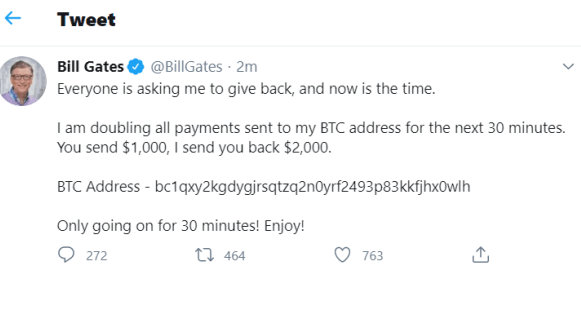
\includegraphics[width=10cm]{bill_hack.png}
  \caption[Screenshot von Bill Gates' Twitter Account während des Hacks]{Screenshot von Bill Gates' Twitter Account während des Hacks\footnotemark}
\end{figure}
\footcitetext{PicTwitterHack}
Genauere Details zu den Umständen des Hacks wurden von Twitter aufgrund von Sicherheitsrisiken nicht veröffentlicht. 
\par
Im August 2021 wurden dann vier Personen verhaftet, darunter der damals noch 17-jährige Graham Ivan Clark, 
der die Spear-Phishing-Attacke initiierte. Ein 19-jähriger führte zusammen mit einem 22-jährigen den 
Bitcoin-Scam aus, während ein weiterer 22-jähriger Graham bei der Umsetzung des Angriffs unterstützte.\footcite{teampw_TwitterPhishing}\\


\section{Bezug zum Ethischen Hacking}
Nach den oben genannten Definitionen und Beispielen stellt sich die Frage: Wenn diese Taktiken
so schädlich sind, warum werden sie dann von Sicherheitsexperten eingesetzt? Hierbei hilft das Konzept
des \textbf{Ethischen Hackings}, und der erste Schritt zum Verständnis führt über das sogenannte
\textbf{Penetration Testing} (auch \textbf{Pentesting} genannt).

\subsection{Pentesting von Social Engineering}
Beim Pentesting geht es darum, die Sicherheit eines Systems durch genehmigte Einbruchsübungen auf die 
Probe zu stellen. Hierhei geht es nicht darum, Schaden anzurichten, sondern potentielle Schwachstellen
noch vor Angreifern zu identifizieren und weitesgehend zu schließen.
\par
Dazu beauftragen Unternehmen Sicherheitsexperten, welche die eigenen Systeme auf Schwachstellen untersuchen.
Dazu nutzen sie die gleichen Methoden und Werkzeuge, welche auch Angreifer verwenden würden. Pentesting gibt
es oft in technischen Formen, wie zum Beispiel das Ausnutzen von Schwachstellen in Software oder Hardware,
allerdings auch sehr häufig in Form von Social Engineering und Phishing.
\par
Ein Bespiel hierfür wäre, wenn ein Pentester eine E-Mail, welche vermeindlich von der IT-Abteilung stammt,
mit einem Link an die Mitarbeiter des Unternehmens schickt. Jedoch führt der Link zu keiner schädlichen Webseite, sondern
zu einer Informationsseite, in welcher erklärt ist, dass es sich um einen Test handelt. Dadurch wird 
den Mitarbeitern gleichzeitig gezeigt, wie leicht solche Angriffe umsetzbar sind, ohne wirtschaftlichen Schaden
anzurichten. Im Anschluss an solche Tests werden dann alle Daten ausgewertet und, falls nötig, mehrere Schulungen angeboten.

\subsection{Rolle von Ethik und Moral}
Durch die harmlose Intension hinter Pentesting kann man auf ersten Blick meinen, Menschen als Versuchsobjekte
zu benutzen wäre moralisch und ethisch vertretbar. Allerdings muss hier beachtet werden, dass der 
einzige Unterschied zwischen einem ethischen Hacker und einem Angreifer der \textbf{Kontext} ist.
Ethisch betrachtet täuscht man hier bereitwillig Menschen, nur um einem guten Zweck zu dienen. 
\par
Hierzu muss man das \textbf{Prinzip des minimalen Schadens} als oberste ethische Regel betrachten. So sollten
Personen, die in dem Test geprüft werden, keineswegs gedemütigt werden. Zudem soll keine Angst oder Panik
verbreitet werden. So sollte die E-Mail keine gefälschte Kündigung enthalten, sondern zum Beispiel die 
Ankündigung eines neuen Sicherheitssystems. Zudem sollten durch die Tests kein Datenverlust entstehen.
\par
Man kann auch in der Herangehensweise gewisse Züge des \textbf{Utilitarismus} erkennen. Diese Lehre besagt,
dass eine Handlung exakt dann moralisch richtig ist, wenn das höhere Wohl aller Beteiligten dadurch gefördert.
Dadurch lassen sich Pentests an Menschen sehr leicht rechtfertigen, da genau diese Absicht verfolgt wird.
\par
Eine vollständige \textbf{Aufklärung} ist nach den Tests unabdingbar. Alle Beteiligten sollen danach
erfahren, dass es sich um einen Test gehandelt hat, was der Ziel hinter denen war und welche Maßnahmen
jeder Einzelne ergreifen kann, damit er nicht Opfer eines tatsächlichen Angriffs wird.
Die Mitarbeiter sollen sich nach den Tests sicherer und informierter fühlen, anstatt verunsichert und 
verängstigt.
\par
Die Auswertung der Tests sollte auch unter jeden Umständen anonmyisiert erfolgen. Es geht nur um
die statistische Auswertung, nicht die Beurteilung jedes Einzelnen. 

\subsection{Rechtliche Rahmenbedingungen}
Nachdem die ethischen Aspekte dargelegt wurden, stellt sich noch die Frage, in welcher Form solche 
Pentests legal durchgeführt werden können. In Deutschland gilt erstmal das Hacking-Verbot und wird 
im Strafgesetzbuch (StGB) unter Strafe gestellt. Für ethische Hacker sind vor allem die  
sogenannten \textbf{Hackerparagraphen} von Bedeutung, die in § 202a bis § 202c StGB und § 303 StGB zu finden sind.
\par
Während § 202a StGB das Ausspähen von Daten, § 202b StGB das Abfangen von Daten und § 202c StGB 
die Vorbereitung auf das Ausspähen und Abfangen von Daten unter Strafe stellt, halten diese Paragraphen
primär erstmal keine Ausnahmen für ethische Hacker bereit. Was allerdings auch hier von Relevan ist, 
ist die \textbf{Einwilligung des Betroffenen}. Diese ist unerlässlich, damit ethische Hacker legal arbeiten können.
Alle ethischen Hacker müssen sich also vorab jeglicher Arbeit vertraglich absichern, sodass sie im 
Falle eines Rechtsstreits beweisen können, dass sie die Erlaubnis des Betroffenen hatten. Dort werden alle
Rahmenbedingungen, also Prüfungsumfang, Dauer, Art der Tests, Zielgruppe, Verschwiegenheit, etc., an die sich der Hacker 
unter allen Umständen halten muss, festgehalten.
\par
Abschließend kann man also festhalten, dass man ohne Vetrag kein Pentesting durchführen darf. Erst die vorherige
schriftliche und präzise Einwilligung des Rechteinhabers legalisiert das ethische Hacken. Und diese Einwilligung
ist auch die Mauer, welche sogennante \textbf{Black-Hat-Hacker} von \textbf{White-Hat-Hackern} trennt.\\


\section{Ausblick}

% TODO
\subsection{Bedeutung von Präventionsmaßnahmen und Sensibilisierung}
Jeder denkt, er würde niemals auf solche Angriffe hereinfallen. Doch die Realität statistisch gesehen
anders aus. IT-Schutzmechanismen helfen nur bedingt, also muss die Sicherheitslücke beim Menschen
geschlossen werdne. Ausschließlich Präventionsmaßnahmen in Form von Schulungen jeglicher Art können
zur Sensibilisierung potentieller Opfer beitragen. Inhalt sollte unter anderem beinhalten, dass
nur vertrauliche Quellen angeklickt werden, oder auch allgemein, dass Daten nicht leichtfertig
weitergegeben werden sollten. Ältere Menschen sollten zudem zum Beispiel von Banken aufmerksam gemacht
werden, wenn andere Personen anrufen und hohe Geldsummen an Gutscheinkarten verlangen.

\subsection{Zukünftige Entwicklungen und Herausforderungen}
Vor allem macht künstliche Intelligenz es Opfern immer schwerer, Angriffe zu erkennen. Stimmen können
unbemerkbar imitiert werden, Texte können so geschrieben werdne, als wären sie von der eigentlichen Person.
Zudem können Angriffe durch KI-Tools automatisiert werden, sodass die generelle Menge an Angriffen
steigt. Deswegen wird es immer wichtiger, dass Menschen sich mit der Thematik auseinandersetzen und präventiv
lernen, wie man sich schützen kann.

%----------------------------------------------------------------------------------------
\clearpage
\printbibliography[title={Literaturverzeichnis}]

\end{document}